\documentclass[11pt,letterpaper]{article}
\usepackage[letterpaper,margin=0.79in,headheight=15pt,headsep=18pt,footskip=25pt]{geometry}
\usepackage[T1]{fontenc}
\usepackage{amsmath,amsthm,amssymb}
\usepackage{lmodern,microtype}
\usepackage{enumitem,booktabs,tabularx,array,ragged2e}
\usepackage{graphicx,xcolor,tikz}
\usetikzlibrary{arrows.meta,positioning,calc}
\usepackage{listings,fancyhdr,lastpage,titlesec,caption,needspace,placeins}
\usepackage[hidelinks,breaklinks=true]{hyperref}
\usepackage{url}
\hypersetup{pdftitle={Ghost Portal Cartographer: Evidence-Tiered Mapping of Indirect Sensitive-Data Egress},pdfauthor={Thor Thor},pdfsubject={Reproducible security research manuscript and read-only synthetic reference algorithm},pdfkeywords={data lineage, information flow, provenance, observability, indirect egress, uncertainty}}
\definecolor{ink}{gray}{0.08}
\color{ink}
\pagestyle{fancy}
\fancyhf{}
\fancyhead[L]{\footnotesize\textsc{Ghost Portal Cartographer}}
\fancyhead[R]{\footnotesize\textsc{Thor}}
\fancyfoot[C]{\footnotesize \thepage}
\renewcommand{\headrulewidth}{0pt}
\renewcommand{\footrulewidth}{0pt}
\titleformat{\section}{\large\bfseries}{\thesection.}{0.55em}{}
\titleformat{\subsection}{\normalsize\bfseries}{\thesubsection}{0.6em}{}
\titlespacing*{\section}{0pt}{13pt plus 2pt minus 2pt}{6pt}
\titlespacing*{\subsection}{0pt}{10pt plus 1pt minus 1pt}{4pt}
\captionsetup{font=small,labelfont=bf,justification=justified,singlelinecheck=true}
\setlength{\parindent}{0pt}
\setlength{\parskip}{5.0pt plus 1pt minus 1pt}
\emergencystretch=2em
\sloppy
\setlist[itemize]{topsep=3pt,itemsep=1pt,parsep=0pt,leftmargin=1.35em}
\setlist[enumerate]{topsep=3pt,itemsep=2pt,parsep=0pt,leftmargin=1.55em}
\newtheorem{definition}{Definition}
\newtheorem{proposition}{Proposition}
\newtheorem{lemma}{Lemma}
\newtheorem{corollary}{Corollary}
\newtheorem{remark}{Remark}
\newcommand{\code}[1]{\texttt{#1}}
\newcolumntype{L}{>{\raggedright\arraybackslash}X}
\newcommand{\st}[1]{\texttt{\scriptsize #1}}
\newcommand{\dom}{\operatorname{dom}}
\newcommand{\OO}{\mathsf{O}}
\newcommand{\RR}{\mathsf{R}}
\newcommand{\PP}{\mathsf{P}}
\lstset{basicstyle=\ttfamily\footnotesize,frame=single,framesep=6pt,breaklines=true,columns=fullflexible,keepspaces=true,showstringspaces=false,upquote=true}
\begin{document}
\thispagestyle{empty}
\begin{center}
{\LARGE\bfseries Ghost Portal Cartographer\par}
\vspace{0.45em}
{\large Evidence-Tiered Mapping of Indirect Sensitive-Data Egress\par}
\vspace{1.4em}
{\normalsize Thor Thor\par}
\vspace{0.25em}
{\small Independent Open-Source Researcher, THOR-SEC\par}
{\small ORCID \href{https://orcid.org/0009-0001-6573-385X}{0009-0001-6573-385X} \quad Repository \url{https://github.com/codethor0/ghost-portal-cartographer}\par}
\vspace{0.4em}
{\small Independent research conducted on the author's own time; not sponsored by or representative of an employer.\par}
{\small Research paper, November 2026. Not peer reviewed; open for technical challenge.\par}
\end{center}
\vspace{0.6em}
\begin{abstract}
\small
Sensitive information can cross a security boundary through logs, traces, memory artifacts, caches, backups, and integrations even when the primary application response is protected. Ghost Portal Cartographer (GPC) analyzes these indirect routes as a finite, declared artifact-version graph without inspecting payload contents. Three independently bounded searches distinguish reported scalar-ordered lineage, reported lineage with unresolved order, and possible data or unknown-content reachability. A positive witness survives resource exhaustion in another search, and the selected witness is labeled by the strongest relation it satisfies. Trace parentage remains unauthenticated context, not proof of transferred data. A local HMAC demonstration authenticates declared transformation metadata, bound to the artifacts and trust domains it describes, under a test policy; it cannot establish sanitization or exclude a candidate route. The standard-library implementation was evaluated on synthetic graphs using 171 tests, two separately coded graph oracles, exhaustive small-graph cases, randomized comparisons, and eleven detected deliberate mutations. These results support graph-relative search properties under stated assumptions; they do not establish verified exfiltration, complete observation, formal verification, or production readiness. Code, fixtures, and falsification conditions accompany the paper.
\end{abstract}
\noindent{\small\textbf{Keywords:} indirect data egress; evidence-tiered lineage; provenance; bounded graph search; observability; reproducibility.}

\begin{center}
\vspace{0.6em}
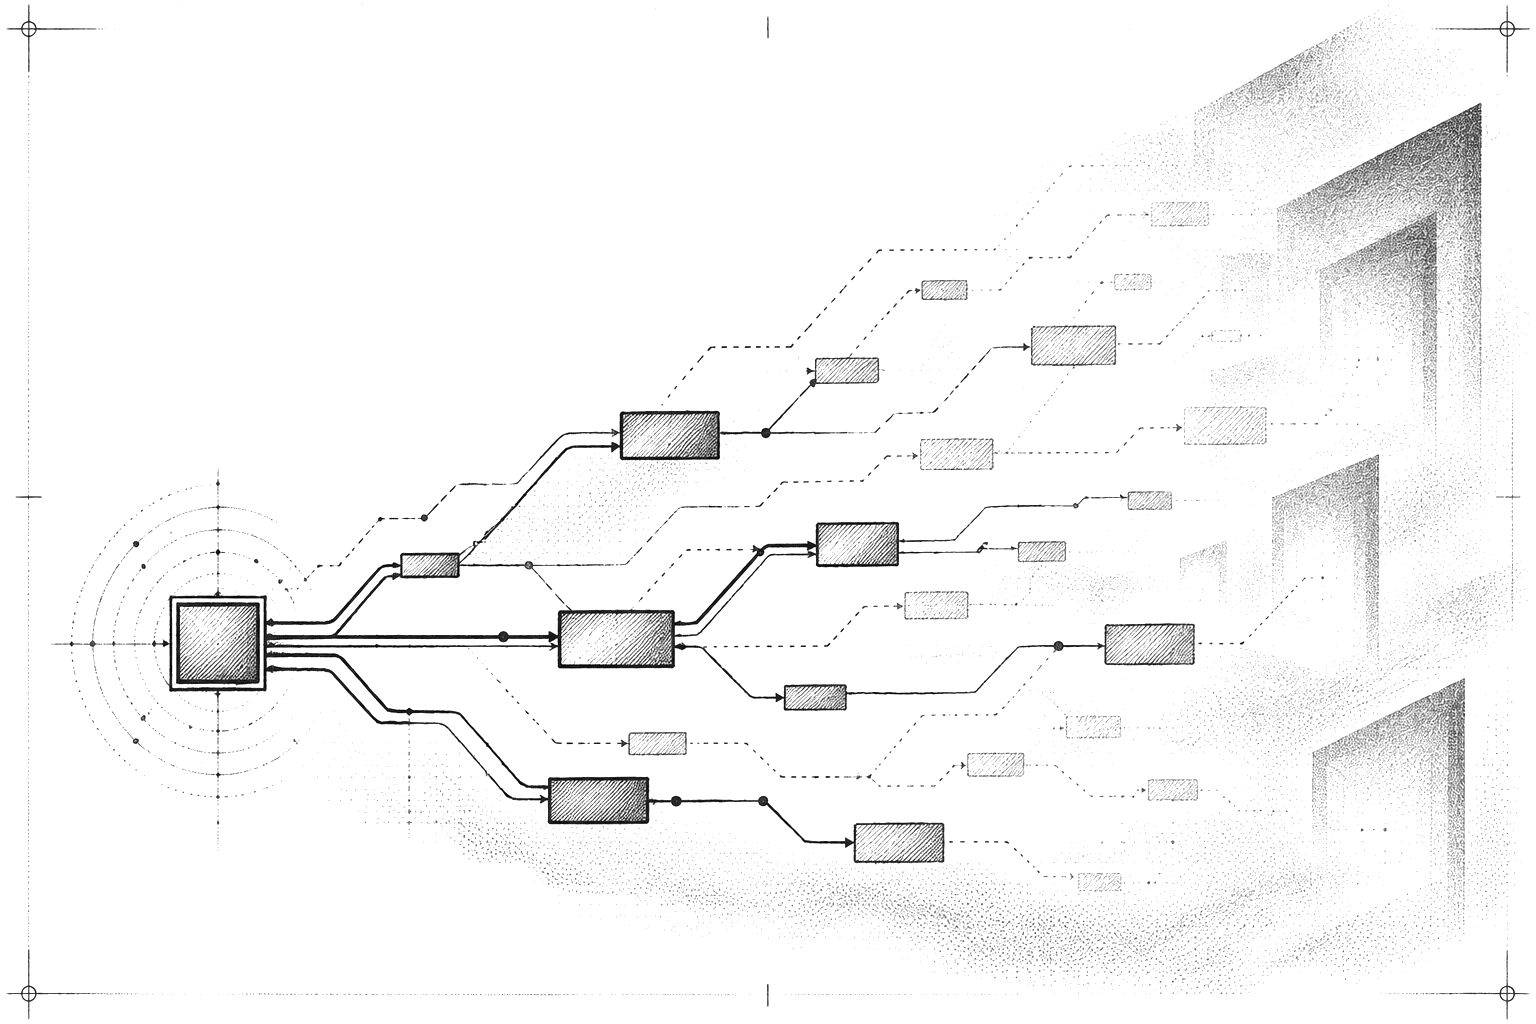
\includegraphics[width=0.74\textwidth]{GPC_Conceptual_Cover.png}\par
\vspace{0.35em}
\begin{minipage}{0.74\textwidth}\footnotesize\centering
Conceptual illustration of candidate artifact routes across an observation boundary; not an empirical flow trace or a results figure.
\end{minipage}
\end{center}
\clearpage

\section{Problem and research question}
A protected response is not the end of a data lifecycle. Its contents may reappear in exception logs, distributed-trace attributes, diagnostic memory snapshots, application caches, and configured exports. OWASP advises against exposing secrets in logs, and OpenTelemetry documents the risk of capturing private values in telemetry \cite{owasp_logging,otel_sensitive}. MITRE separately records weaknesses involving sensitive logs and cached information \cite{cwe532,cwe524}, and a 2026 empirical study of Android application logs reports private information written to logs in practice \cite{androidlogs}. These mechanisms differ operationally, but each can create another artifact outside the original control boundary.

A dependency diagram alone cannot establish what moved. A shared trace ID is not an artifact-derivation record. An enabled exporter is not proof of transmission. Missing telemetry is not proof of safety. Any useful analysis must separate artifact identity, reported evidence, order, provenance, inventory coverage, and policy before it assigns a result.

\textbf{Research question.} Can an auditable, metadata-only graph procedure retain reported paths and expose what remains unknown, without reading sensitive payloads or treating missing observations as proof that no route exists?

Table~\ref{tab:surfaces} lists the surfaces considered here.

\textbf{Scope.} The result is a tested decision procedure for a supplied finite graph. It is not a runtime collector, a data-loss prevention product, a cryptographic provenance system, a content-aware taint engine, or proof that a deleted artifact was purged. An edge labeled \code{observed} remains a claim supplied by an input source.

\section{Contributions and relationship to prior work}
GPC separates three questions that are often collapsed into one alert: Does a possible route exist? Is that route backed by reported artifact relationships? Do the reported scalar sequences admit a strict order? Three independently budgeted searches answer those questions while retaining stronger positive witnesses, even if a broader search hits a cap. The output also records path-specific policy, declared coverage gaps, and diagnostic provenance claims. Predecessor pointers bound path-storage costs. The contribution is the combination of these decision semantics and an executable test artifact, not a claim to have invented graph search, cryptographic authentication, or dynamic taint analysis.

Prior systems address important parts of this problem. W3C PROV-DM defines a provenance vocabulary; CamFlow records system-wide provenance; TaintDroid follows information flow at runtime; OpenLineage standardizes lineage events for data workflows \cite{prov,camflow,taintdroid,openlineage}. GPC does not collect or authenticate their evidence. OWASP, OpenTelemetry, MITRE, and NIST describe the security risks of records and retained information \cite{owasp_logging,otel_sensitive,nist_logging}. RIFT studies pre-commit information-flow edge admission; GPC instead evaluates paths already declared in an input graph \cite{rift}. W3C Trace Context and OpenTelemetry provide context propagation, not proof that bytes crossed a boundary \cite{w3ctrace,otelapi}. The in-toto framework and DSSE distinguish authenticated statements from the truth of their contents \cite{intoto,dsse}. Lamport's work explains why distributed order is not reducible to wall-clock time \cite{lamport}. Provenance-based attack investigation is the closest technical community. Backtracking from a detection point through operating-system dependency graphs dates to King and Chen \cite{kingchen}; SPADE collects distributed provenance \cite{spade}; HOLMES correlates suspicious information flows into attack stages \cite{holmes}; NoDoze and UNICORN rank or learn from provenance paths to reduce false alarms \cite{nodoze,unicorn}. NovaFabric records agent runs as signed evidence bundles whose lineage edges are marked as observed or inferred \cite{novafabric}, a two-class distinction close to GPC's mode field. Patent publications describe taint sets over provenance graphs built from audit records \cite{pat_sri}, lineage graphs with sensitive-element classification across streaming platforms \cite{pat_jpm}, and time-ordered lineage for threat detection \cite{pat_tannin}. Those systems build and score graphs from collected events. GPC instead takes a declared graph as given and separates how strongly each returned route is supported, under explicit search budgets.

The term \emph{declassification} follows the information-flow literature \cite{denning,sabelfeldmyers}, where releasing information is characterized by what is released, by whom, where and when \cite{sabelfeldsands}. GPC deliberately gives a declassification claim no release effect at all: it is recorded and, when possible, authenticated, but never removes an edge. Bounded verification that reports an unknown outcome rather than safety when a bound is reached is established practice in model checking \cite{bmc}; GPC applies that discipline to three nested relations searched independently. The present work is a reproducible systems synthesis whose value depends on the limits it makes visible, not an assertion that earlier approaches are inferior.

\section{Threat, trust, and observation boundary}
\subsection{Protected artifacts, trust domains, and policy}
The query names a source artifact \(s\), a declared sensitivity category \(c\), and a destination trust domain \(d\). GPC does not inspect bytes to confirm the category, and category does not change reachability. The independent policy function is \(A(c,d)\in\{\mathsf{DENIED},\mathsf{PERMITTED},\mathsf{UNSPECIFIED}\}\). An absent rule yields \(\mathsf{UNSPECIFIED}\), not implicit permission. Intermediate assessments describe only the returned witness path; they are not a regulatory or global authorization decision.

A trust domain is an ownership, authority, or processing boundary rather than a geographic location. A reported path to a vendor domain is not itself proof that an unauthorized person viewed the content. Conversely, a supposedly internal destination can still be disallowed by policy.

\subsection{Adversaries and collection failures}
The adversary may influence instrumentation, metadata, or inventory. The relevant failures include copied secrets in logs, retained diagnostic artifacts, forged locators, reordered sequences, missing collectors, hidden destinations, and unrecorded historical copies. The kernel validates declared structure; it cannot verify that a malicious input describes reality. W3C trace context may originate beyond a trusted boundary \cite{w3ctrace}. A fabricated edge can create a false route; an omitted edge can hide a real one. Those are limits of input trust, not defects that graph traversal alone can overcome.

\subsection{Data surfaces and evidence}
\begin{table}[htbp]
\centering\small
\caption{Indirect-copy surfaces and the evidence question each leaves open.}
\label{tab:surfaces}
\begin{tabularx}{\textwidth}{@{}p{1.04in}L L@{}}
\toprule
\textbf{Surface} & \textbf{Candidate derived artifact} & \textbf{Unresolved evidence question}\\
\midrule
Logs & Exceptions, URL or body fragments, serialized context & Does the record actually contain the declared category?\\
Telemetry / traces & Exported spans, metrics, attributes, baggage & Does a shared ID indicate derivation or only correlation?\\
Memory & Heap snapshot, dump, support bundle & Was it retained, transferred, or made accessible?\\
Caches & Browser, application, CDN, distributed cache entry & Did expiry or deletion remove every prior copy?\\
Integrations & Webhook payload, support upload, partner export & Was the configured route actually invoked?\\
Backups / archives & Object versions, copied logs, replicas & What historical or onward copies remain?\\
\bottomrule
\end{tabularx}
\end{table}

\section{Typed graph and three evidence tiers}
\begin{definition}[Declared artifact-version graph]
A finite directed graph \(G=(V,E)\) has unique artifact-version identifiers \(v\in V\), each with declared domain \(\dom(v)\), surface \(\operatorname{surf}(v)\), inventory annotation \(\operatorname{cov}(v)\in\{\mathsf{complete},\mathsf{partial},\mathsf{unknown}\}\), and an optional \emph{declared} SHA-256 digest \(h(v)\). Neither a claimed complete inventory nor an input digest establishes that physical artifact bytes were checked.
\end{definition}

\begin{definition}[Candidate lineage and transformation claims]
An edge \(e=(id,u,v,m,f,\sigma,r,\kappa,\tau,a)\) connects declared artifact versions. Mode \(m\in\{\mathsf{observed},\mathsf{inferred}\}\), flow type \(f\in\{\mathsf{data},\mathsf{unknown},\mathsf{control},\mathsf{declassified}\}\), optional scalar sequence \(\sigma\), and evidence locator \(r\) are input claims. Optional \(\kappa\) is a claimed predecessor edge ID; \(\tau(e)=(\operatorname{traceID}(e),\operatorname{spanID}(e),\operatorname{parentSpanID}(e))\) comprises three optional trace/span identifiers; \(a\) carries a transformation claim. None of \(\kappa, \tau, a\), or a locator authenticates a collector.
\end{definition}

Define candidate relations conservatively:
\begin{align}
E_P &= \{e\in E : f(e)\in\{\mathsf{data},\mathsf{unknown},\mathsf{declassified}\}\}, \label{eq:possible}\\
E_R &= \{e\in E_P : m(e)=\mathsf{observed},\ f(e)\in\{\mathsf{data},\mathsf{declassified}\},\ \operatorname{nonblank}(r(e))\}, \label{eq:reported}\\
E_O &= \{e\in E_R : \sigma(e)\ne\bot\}.\label{eq:orderededge}
\end{align}
Thus \(E_O\subseteq E_R\subseteq E_P\). For an admissible query \(q=(s,c,d)\), \(d\ne\dom(s)\), predicate \(\PP(q)\) means there is a directed path in \(E_P\) from \(s\) to a different vertex in domain \(d\); \(\RR(q)\) means one exists in \(E_R\); and \(\OO(q)\) additionally requires a path in \(E_O\) whose edges satisfy
\begin{equation}
\sigma(e_1)<\sigma(e_2)<\cdots<\sigma(e_k).\label{eq:strict}
\end{equation}
A strictly increasing scalar sequence is a property of declared metadata, not authenticated distributed causality. \(\RR(q)\) does not require sequence order: missing, repeated, or inverted values can invalidate an ordered finding without discarding the reported graph path. Category \(c\) determines policy lookup and claim diagnostics; it does not verify payload content. Figure~\ref{fig:map} shows the fixture used in Section~\ref{sec:examples}.

\begin{figure}[htbp]
\centering
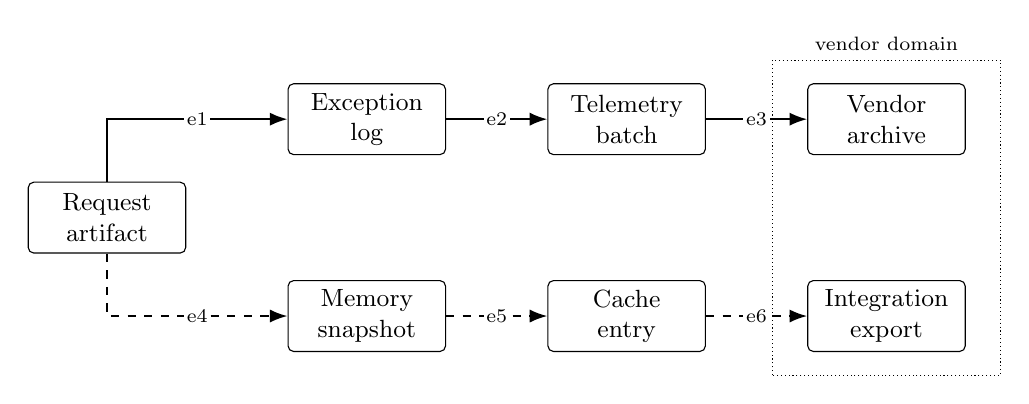
\begin{tikzpicture}[>=Latex, box/.style={draw=black,rounded corners=2pt,minimum height=9mm,minimum width=20mm,align=center,font=\small,inner sep=3pt}, obs/.style={->,line width=0.75pt}, hyp/.style={->,dashed,line width=0.75pt}, lab/.style={font=\scriptsize,fill=white,inner sep=1pt}]
\node[box] (app) at (0,0) {Request\\artifact};
\node[box] (log) at (3.3,1.25) {Exception\\log};
\node[box] (tele) at (6.6,1.25) {Telemetry\\batch};
\node[box] (vendor) at (9.9,1.25) {Vendor\\archive};
\node[box] (memory) at (3.3,-1.25) {Memory\\snapshot};
\node[box] (cache) at (6.6,-1.25) {Cache\\entry};
\node[box] (export) at (9.9,-1.25) {Integration\\export};
\draw[obs] (app.north) |- node[lab,pos=0.75]{e1} (log.west);
\draw[obs] (log.east) -- node[lab]{e2} (tele.west);
\draw[obs] (tele.east) -- node[lab]{e3} (vendor.west);
\draw[hyp] (app.south) |- node[lab,pos=0.75]{e4} (memory.west);
\draw[hyp] (memory.east) -- node[lab]{e5} (cache.west);
\draw[hyp] (cache.east) -- node[lab]{e6} (export.west);
\draw[densely dotted] (8.45,-2.0) rectangle (11.35,2.0);
\node[font=\scriptsize,anchor=south] at (9.9,2.0) {vendor domain};
\end{tikzpicture}
\caption{The fictional two-lane fixture. Both sinks are in the vendor trust domain. Solid lines encode input-reported data-derivation claims; dashed lines are inferred data or unknown-content relationships.}
\label{fig:map}
\end{figure}

\section{Reported causal context and conservative declassification}
\subsection{Context matching does not authenticate data transfer}
For consecutive reported path edges \((e_i,e_{i+1})\), define an optional \emph{claimed edge-parent match}
\begin{equation}
C_{\mathrm{claim}}(e_i,e_{i+1})\equiv [\kappa(e_{i+1})=id(e_i)].\label{eq:context}
\end{equation}
For all three components of \(\tau(e)\), \(\bot\) denotes absence. When supplied, trace IDs and span IDs are respectively 32 and 16 lowercase hexadecimal characters, and all-zero values, which W3C Trace Context defines as invalid, are rejected \cite{w3ctrace}; a parent span requires a declared trace and current span. These identifiers are the context-propagation fields of distributed tracing \cite{otel_context}. For consecutive reported edges, a claimed span-parent match is
\begin{align}
S_{\mathrm{claim}}(e_i,e_{i+1})\equiv{}&[\kappa(e_{i+1})=\bot]\ \land\ [\operatorname{parentSpanID}(e_{i+1})\ne\bot] \notag\\
&\land\ [\operatorname{traceID}(e_i)=\operatorname{traceID}(e_{i+1})\ne\bot] \notag\\
&\land\ [\operatorname{spanID}(e_i)=\operatorname{parentSpanID}(e_{i+1})\ne\bot].\label{eq:spanmatch}
\end{align}
The reference code evaluates the claimed edge-parent identifier first, if present, reporting \code{MATCHED\_UNAUTHENTICATED\_PARENT} or \code{CONFLICTING\_PARENT}. Only when that identifier is absent does it evaluate a supplied parent-span identifier, reporting \code{TRACE\_PARENT\_MATCH}, \code{TRACE\_PARENT\_MISMATCH}, or \code{UNSCOPED\_TRACE} if the preceding span or trace is absent. When neither parent field is present, it reports \code{NO\_PARENT\_CLAIM}. These are diagnostic annotations, not transition guards. In particular, \(C_{\mathrm{claim}}\) and \(S_{\mathrm{claim}}\) do \emph{not} relax Equation~\eqref{eq:strict} or upgrade \st{REPORTED\_ORDER\_UNRESOLVED} to \st{REPORTED\_ORDERED\_LINEAGE}. A forged identifier can satisfy either predicate, so neither authenticates sensitive-byte transfer \cite{w3ctrace,otelapi}.

\begin{lemma}[Parentage has no admissibility effect]\label{lem:parent}
For consecutive reported edges \(e_i,e_{i+1}\) on a candidate ordered route,
neither claimed edge parentage \(C_{\mathrm{claim}}(e_i,e_{i+1})\) nor claimed
span parentage \(S_{\mathrm{claim}}(e_i,e_{i+1})\) changes admission to
\textup{\textsc{OrderedRoute}}. Admission depends only on membership in \(E_O\) and
\(\sigma(e_{i+1})>\sigma(e_i)\), with \(\sigma(e_0)\) read as the start sentinel \(-1\).
\end{lemma}
\begin{proof}
The transition guard is Equation~\eqref{eq:strict}, and
neither Equation~\eqref{eq:context} nor Equation~\eqref{eq:spanmatch} occurs
in that guard or in the witness re-verification of Section~\ref{sec:search}. These annotations cannot upgrade an inverted or absent
sequence to \st{REPORTED\_ORDERED\_LINEAGE}.
\end{proof}

\subsection{HMAC demonstration authenticates statements, not sanitization}
A \(\mathsf{declassified}\) edge may carry a bounded claim with attester and policy IDs, category, transform name, source/output declared digests, nonce, validity window, and MAC. For an in-process trust configuration \(T\), category \(c\), and explicit verification epoch \(t\), the demonstration reports metadata authentication only when
\begin{align}
M_T(e,c,t) \equiv {} & \mathrm{MACValid}_T(a(e),e)\ \land\ \mathrm{Authorized}_T(\mathrm{attester},\mathrm{policy},c,\mathrm{transform}) \notag\\
&\land\ h(u)=a.\mathrm{sourceDigest}\ \land\ h(v)=a.\mathrm{outputDigest} \notag\\
&\land\ a.\mathrm{issuedAt}\le t\le a.\mathrm{expiresAt}\ \land\ \mathrm{NonceFirst}_G(e).\label{eq:mac}
\end{align}
For this local model \(\mathrm{MACValid}\) means HMAC-SHA256 over deterministic JSON with a fixed domain-separation prefix, verified using constant-time tag comparison. The caller supplies a test trust mapping \code{attestation\_trust} (\code{attester\_id} to an in-process \code{AttestationTrust} record containing an HMAC key, policy ID, categories and transforms) and an explicit integer \code{verification\_epoch} to the \code{Cartographer} constructor. Neither the key nor the trust mapping is accepted from graph JSON or returned in the result. Missing trust configuration produces \code{UNVERIFIED\_CLAIM} with reason \code{UNTRUSTED\_ATTESTER}; absent verification epoch is also unverified. This is a caller-controlled demonstration, not an operational key-distribution, rotation, revocation or custody system.

\begin{definition}[HMAC validity in the local demonstration]\label{def:mac}
Let \(K\) be a test HMAC key selected from an in-process trust configuration \(T\),
let \(\mathrm{DSP}\) be the fixed domain-separation prefix, let
\(\beta(e)=(u,v,\dom(u),\dom(v))\) be the source and output artifact versions of the edge carrying the claim together with their declared domains, and let
\(\mathrm{canonical}(a\setminus\{\mathrm{mac\_hex}\},\beta(e))\) denote deterministic JSON
serialization of the claim fields \emph{excluding} its MAC field, extended with \(\beta(e)\). Define
\begin{equation}
\begin{aligned}
\mathrm{MACValid}_{T}(a,e)\equiv\mathrm{ct\mbox{-}eq}\big(&\mathrm{HMAC\mbox{-}SHA256}_{K}(\\[-2pt]
&\mathrm{DSP}\,\|\,\mathrm{canonical}(a\setminus\{\mathrm{mac\_hex}\},\beta(e))),\; a.\mathrm{mac\_hex}\big).
\end{aligned}
\label{eq:macvalid}
\end{equation}
\end{definition}
Here \(\mathrm{ct\mbox{-}eq}\) compares the computed hexadecimal tag using
constant-time comparison. The code uses \code{hmac.compare\_digest} and the
literal prefix \code{GPC-DECLASSIFICATION-HMAC-DEMO} followed by a zero byte.
Binding \(\beta(e)\) means a claim issued for one artifact pair cannot authenticate on an edge between different artifacts or across a different trust boundary, in the same spirit as the subject binding of an in-toto statement \cite{intoto}. The tag is checked immediately after the attester lookup, before any field-specific reason is reported. This is symmetric message authentication.

The predicate \(\mathrm{NonceFirst}_G(e)\) is scoped to one \code{analyze} invocation: after sorting declassified edges by edge ID, the first edge with an \((\mathrm{attesterID},\mathrm{nonce})\) pair is assessed, and subsequent edges with that pair are marked \code{DUPLICATE\_NONCE\_IN\_GRAPH}, even when the first claim fails a later validation. A fresh nonce set is used at every call. Thus replay across invocations, processes or archives is \emph{not detected}; the demonstration does not persist anti-replay state. An authenticated claim binds \emph{supplied metadata} relative to a test key. Declared digests are not independently measured against bytes; freshness is a caller-supplied epoch. This is \emph{not} DSSE, an in-toto verifier, a public-key signature, a production trust system, or proof that an output no longer contains sensitive content \cite{intoto,dsse}.

Most importantly, even when Equation~\eqref{eq:mac} holds, effective category-specific sanitization is \emph{not} established. Therefore the executable kernel applies no declassification-based flow suppression:
\begin{equation}
\forall e\in E_P,\ \forall c,\quad \mathrm{ExcludeForClaim}(e,c)=\mathsf{false}.\label{eq:nosuppress}
\end{equation}
For otherwise identical edge metadata, \(f(e)=\mathsf{declassified}\) and \(f(e)=\mathsf{data}\) have identical membership in \(E_P\), \(E_R\), and \(E_O\): a valid HMAC does \emph{not} change route existence or the primary result. Only the separate claim-assessment diagnostics differ. The code reports \st{AUTHENTICATED\_METADATA\_CLAIM} or \st{UNVERIFIED\_CLAIM}; missing claims, wrong MACs, expired validity, different categories, policy mismatch, incorrect declared digests, and repeated nonces cannot remove a candidate route. A \emph{syntactically malformed} claim (for example a non-hexadecimal tag or an inverted validity window) is treated differently: the loader rejects the entire input with an error, so no partial result is produced. This fails closed, but it also means one malformed claim from any party prevents analysis until the input is corrected. Assessments cover every declassified edge in the supplied graph, not only edges on the selected witness. A future category-specific exclusion would additionally require a trustworthy semantic postcondition for the transformation and a model of other residual channels, neither supplied here. An individual IETF Internet-Draft discussing transformation evidence is relevant context, not an endorsed standard or proof of sanitization \cite{drafttransform}.

\begin{lemma}[Declassified edges behave as data for path existence]\label{lem:declass}
In the implemented model, an edge \(e\) with \(f(e)=\mathsf{declassified}\)
has identical membership in \(E_P,E_R,E_O\) to an otherwise identical
edge \(e'\) with \(f(e')=\mathsf{data}\).
\end{lemma}
\begin{proof}
Equation~\eqref{eq:possible} admits both flow types;
Equation~\eqref{eq:reported} admits both when the mode and locator requirements
hold; and Equation~\eqref{eq:orderededge} adds only a scalar-sequence filter.
Equation~\eqref{eq:nosuppress} rules out authentication-dependent edge
exclusion. The resulting path-existence predicates are identical, although
diagnostic metadata may differ.
\end{proof}

\section{Independent bounded searches and decision semantics}\label{sec:search}
GPC runs three independent breadth-first searches: \textup{\textsc{OrderedRoute}} on \(E_O\) with state \((v,\sigma_{last})\) and Equation~\eqref{eq:strict}; \textup{\textsc{ReportedRoute}} on \(E_R\) with vertex state; and \textup{\textsc{PossibleRoute}} on \(E_P\) with vertex state. All use parent pointers \(\pi(x)=(x_{parent},edge\_id)\) to reconstruct a witness \emph{once after success}, rather than copying path tuples at every expansion. \textup{\textsc{OrderedRoute}} must not merge states solely by vertex because their future admissible sequences differ.

Each search is independently capped at a positive integer \(b\) of dequeued states. The result contains a witness if one was found, resolution and exhaustion flags, the limit flag, popped and discovered counts, and coverage gaps on visited vertices. A found path proves existence within its declared relation even if additional queued states remain. A limit reached without a path says only that exploration was incomplete.

The selector takes the first returned witness in the order ordered, reported, possible, and then re-verifies that one path against the stronger predicates: edge eligibility and, for the ordered tier, Equation~\eqref{eq:strict} on its own edges. A reported-search witness whose sequences already increase strictly therefore receives \st{REPORTED\_ORDERED\_LINEAGE}, even if the ordered search reached its cap first; the result records \code{witness\_source} and \code{witness\_reclassified}. Re-verification inspects only the returned edges and never consults parentage or claims. If no witness was returned and the possible search finished, the result is \st{NO\_ROUTE\_IN\_DECLARED\_GRAPH} even when a narrower search was capped, because by Proposition~\ref{prop:containment} no narrower route can exist. Figure~\ref{fig:algorithm} summarizes the procedure, and Tables~\ref{tab:states} and~\ref{tab:diagnostics} list the outputs.

\begin{figure}[htbp]
\begin{lstlisting}
GPC(query, b):
    require destination_domain != domain(source); require b >= 1
    ordered  = BFS_ordered(E_O, source, destination, b)
    reported = BFS_vertex(E_R, source, destination, b)
    possible = BFS_vertex(E_P, source, destination, b)
    # Each search carries its own LIMIT and actual popped count.
    path = first of ordered.path, reported.path, possible.path, or empty
    if path:   status = strongest tier whose predicate path satisfies
                        (ORDERED_LINEAGE > ORDER_UNRESOLVED > POSSIBLE_ROUTE)
    else if possible.exhaustive:  status = NO_ROUTE_IN_DECLARED_GRAPH
    else if any(LIMIT):           status = UNKNOWN_LIMIT
    else:                         status = NO_ROUTE_IN_DECLARED_GRAPH
    policy = explicit_policy(category, destination_domain)
    hops = policies_for_each_selected_path_vertex(path)
    coverage = union_of_gaps_at_popped_vertices()
    causal = unauthenticated_context_annotations(path)
    declass = assess_metadata_MAC_claims_without_edge_removal()
    order_issues = sequence_issues(path) if status == REPORTED_ORDER_UNRESOLVED
    return status, ordered, reported, possible, path, witness_source,
           policy, hops, coverage, examined_counts,
           order_issues, causal, declass, provenance_trust=unauthenticated
\end{lstlisting}
\caption{Abbreviated implementation semantics. A budget-limited broader search cannot erase a narrower positive witness. The full result is composite, not a single loss-prone flag.}
\label{fig:algorithm}
\end{figure}

\begin{table}[htbp]
\centering\small
\caption{Primary result interpretation; individual search outcomes and destination policy remain separately accessible.}
\label{tab:states}
\begin{tabularx}{\textwidth}{@{}p{2.13in}L@{}}
\toprule
\textbf{Primary status} & \textbf{Permitted inference}\\
\midrule
\st{REPORTED\_ORDERED\_LINEAGE} & The selected reference-backed reported witness satisfies the input scalar order. No authenticated causal or payload proof.\\
\st{REPORTED\_ORDER\_UNRESOLVED} & A reported reference-backed witness exists and itself fails strict order (missing, equal, or decreasing values); no ordered witness was returned, possibly because the ordered search was capped.\\
\st{POSSIBLE\_ROUTE} & A data-or-unknown-content path exists in the supplied graph; stronger reported results may be absent or budget-unresolved.\\
\st{NO\_ROUTE\_IN\_DECLARED\_GRAPH} & The possible search finished without a witness; by containment no reported or ordered route exists either. A finite-input statement, never a real-world safety certificate.\\
\st{UNKNOWN\_LIMIT} & No witness was returned and the possible search was capped. Negative conclusions must be withheld.\\
\bottomrule
\end{tabularx}
\end{table}

\begin{table}[htbp]
\centering\small
\caption{Secondary diagnostics are separate from the primary finding; missing entries do not prove trustworthy observation.}
\label{tab:diagnostics}
\begin{tabularx}{\textwidth}{@{}p{1.28in}L@{}}
\toprule
\textbf{Category} & \textbf{Reported diagnostic values}\\
\midrule
\textbf{Order} & \code{MISSING\_SEQUENCE}, \code{NON\_INCREASING\_SEQUENCE}, computed on the selected witness when the status is \st{REPORTED\_ORDER\_UNRESOLVED}; empty for every other status.\\
\textbf{Parent context} & \code{NO\_PARENT\_CLAIM}, \code{MATCHED\_UNAUTHENTICATED\_PARENT}, \code{CONFLICTING\_PARENT}, \code{UNSCOPED\_TRACE}, \code{TRACE\_PARENT\_MATCH}, \code{TRACE\_PARENT\_MISMATCH}. All are unauthenticated.\\
\textbf{Transformation} & \code{AUTHENTICATED\_METADATA\_CLAIM} or \code{UNVERIFIED\_CLAIM}, accompanied by a reason and \code{edge\_suppressed=false}, for every declassified edge in the graph. No status proves sanitization.\\
\textbf{Selection} & \code{witness\_source} (search that returned the path) and \code{witness\_reclassified} (path satisfied a stronger predicate than its search).\\
\bottomrule
\end{tabularx}
\end{table}

\textbf{Policy and coverage.} The destination rule \(A(c,d)\) is returned even if no path exists. For the selected path \((e_1,\ldots,e_k)\), each destination vertex receives its declared-domain policy value. The path annotation is \code{CONTAINS\_DENIED} if any hop is denied; otherwise \code{UNSPECIFIED} if a hop has no rule; otherwise \code{ALL\_PERMITTED}; no path yields \code{NO\_PATH}. These are annotations for \emph{one witness}, not a global property of every route or proof of access control. Coverage reports, in the field \code{declared\_coverage\_gap\_nodes}, list visited vertices whose declared coverage is \code{partial} or \code{unknown}; a self-described complete inventory is not trusted as an audited fact.

\FloatBarrier
\section{Mathematical properties and complexity}
\begin{proposition}[Tier containment]\label{prop:containment}
For every well-formed fixed input graph and admissible query, \(\OO(q)\Rightarrow\RR(q)\Rightarrow\PP(q)\).
\end{proposition}
\begin{proof}
Every ordered route is a path in \(E_O\subseteq E_R\), and every path in \(E_R\) is a path in \(E_P\). All three predicates use the same source and destination-domain condition, and removing the order constraint cannot invalidate existence.
\end{proof}

\noindent\textbf{Scope note (relation versus algorithm).}
Proposition~\ref{prop:containment} is a relation-level implication: \(\OO(q)\Rightarrow\RR(q)
\Rightarrow\PP(q)\) is true independently of budgets. Preserving an
\emph{already returned} witness when a different search reaches
its cap is an algorithm-level property, proved separately by Proposition~\ref{prop:priority}.

\begin{proposition}[Priority preservation under independent limits]\label{prop:priority}
If any search returns a positive witness, no limit flag from a different search can cause the primary result to be \code{UNKNOWN\_LIMIT}. An ordered positive witness is always selected ahead of a reported positive witness, which is selected ahead of a possible positive witness.
\end{proposition}
\begin{proof}
The selector first inspects the three positive path fields in priority order and only inspects cap flags when all fields are empty. Independent cap status therefore cannot replace a previously returned witness. The claim does not say a missing witness in a capped search is absent.
\end{proof}

\begin{corollary}[Strongest-tier labeling of the selected witness]\label{cor:label}
The primary status is the strongest of \(\OO,\RR,\PP\) whose predicate the selected witness itself satisfies, and it is never weaker than the relation of the search that returned that witness.
\end{corollary}
\begin{proof}
By Proposition~\ref{prop:containment} applied to the witness edges, a path satisfying \(\OO\) also satisfies \(\RR\) and \(\PP\), so the tiers are nested and ``strongest satisfied'' is well defined. The selector evaluates the ordered predicate on the selected path first, then the reported predicate, then the possible predicate. A search returns only paths in its own relation, so the search relation is always satisfied. A capped search may still miss a stronger witness that exists elsewhere in the graph; no claim of budget-independent discovery is made.
\end{proof}

\begin{corollary}[Decisive negative]\label{cor:negative}
If the possible search finishes without a witness, then \(\neg\PP(q)\), \(\neg\RR(q)\) and \(\neg\OO(q)\) hold for the supplied graph, whatever the outcome of the other searches.
\end{corollary}
\begin{proof}
Proposition~\ref{prop:exhaustive} gives \(\neg\PP(q)\); the contrapositive of Proposition~\ref{prop:containment} gives the rest.
\end{proof}

\begin{proposition}[Finite-graph exhaustive correctness]\label{prop:exhaustive}
When a search resolves without a cap, \textup{\textsc{PossibleRoute}} decides \(\PP(q)\), \textup{\textsc{ReportedRoute}} decides \(\RR(q)\), and \textup{\textsc{OrderedRoute}} decides \(\OO(q)\) relative to the submitted graph.
\end{proposition}
\begin{proof}
Vertex BFS visits every reachable vertex once and records a predecessor for each newly discovered state. The ordered explorer visits reachable pairs \((v,\sigma_{last})\), accepting exactly edges that satisfy the next strict inequality. Two ordered states with the same vertex and last sequence admit identical possible continuations, so deduplicating that pair is sound for existence. In a finite graph, exhaustion reaches all admissible states. A target is accepted only if its domain is the requested destination and it differs from the source. The ordered search explores walks; existence of an admissible walk and of an admissible path coincide, because removing a closed sub-walk leaves a subsequence of a strictly increasing sequence.
\end{proof}

\begin{lemma}[Returned ordered witnesses are simple]\label{lem:simple}
A witness returned by \textup{\textsc{OrderedRoute}} visits no vertex twice.
\end{lemma}
\begin{proof}
Breadth-first search returns a minimum-hop admissible walk. If such a walk reached \(v\) first with last sequence \(\sigma_1\) and later left \(v\) by edge \(e\) with \(\sigma(e)>\sigma_2>\sigma_1\), then \(e\) would already be admissible at the first visit, giving a strictly shorter admissible walk.
\end{proof}

\begin{proposition}[Edge-addition monotonicity of path existence]
With vertices, domains, query, and existing edge semantics fixed, adding admissible edges cannot remove an already existing \(\PP\), \(\RR\), or \(\OO\) route.
\end{proposition}
\begin{proof}
All original route edges, metadata and sequence order remain available. The added edges enlarge the set of candidate routes without removing existing ones. This does \emph{not} assert monotonicity of finite-budget \emph{discovery}, witness selection, or the primary status under changes to search order or graph size.
\end{proof}

\begin{proposition}[Conservative non-suppression]\label{prop:nonsuppress}
For fixed nodes and reported edges, adding, deleting, authenticating or invalidating well-formed transformation \emph{claims} cannot remove an \(E_P\), \(E_R\), or \(E_O\) path in the implemented model, provided edge types and graph topology themselves remain fixed. A syntactically malformed claim causes the whole input to be rejected rather than any path to be removed.
\end{proposition}
\begin{proof}
Equations~\eqref{eq:possible}--\eqref{eq:orderededge} depend on the declared graph edge type, mode, locator and scalar sequence, but not on Equation~\eqref{eq:mac}. Equation~\eqref{eq:nosuppress} prevents metadata-claim authentication from deleting an admissible edge. Therefore the three path-existence predicates are unaffected by a transformation-claim update. The proposition does not apply to changing an edge's type, topology, locator, sequence, or historical state.
\end{proof}
\textbf{Scope of Proposition~\ref{prop:nonsuppress}.} This is a deliberately narrow invariant of this executable kernel, not a general guarantee for attestation-based declassification. If a future system allowed verified transformations to exclude an edge, a claim update could change its graph membership and the proposition would require a new, status-conditioned statement and proof.

\begin{lemma}[Ordered state-space bound]\label{lem:states}
Let \(E_O\) contain the ordered-eligible edges and let
\textup{\textsc{OrderedRoute}} deduplicate states by \((v,\sigma_{last})\). The number
of distinct reachable search states is at most \(|E_O|+1\).
\end{lemma}
\begin{proof}
The initial state is \((s,-1)\). Every other reachable state
is reached through some edge \(e\in E_O\) and has the form
\((\mathrm{dst}(e),\sigma(e))\). Different edges may yield identical pairs,
but deduplication adds a pair only once. There are at most \(|E_O|\)
non-initial pairs and the initial state.
\end{proof}

\textbf{Complexity.} Let \(n=|V|\), \(m=|E|\). Constructing adjacency lists and deterministic edge-ID ordering takes \(O(n+m\log(m+1))\) time and \(O(n+m)\) memory. Each vertex-only BFS has \(O(n+m)\) time and \(O(n)\) auxiliary state on top of graph storage; parent reconstruction adds \(O(\ell)\) for a witness of length \(\ell\le m\). Every ordered state after the start is uniquely determined by the destination vertex and sequence of a last eligible edge, so at most \(m+1\) such states exist. Re-scanning outgoing edges at different sequence states gives a conservative \(O(n+m^2)\) time bound. Re-verifying the selected witness costs \(O(\ell)\). The popped-state budget does not bound memory: discovered states enter the predecessor map before they are popped. Parent pointers and queues require \(O(n+m)\) graph-plus-search memory, rather than quadratic copied-path memory. Metadata-claim assessment additionally scans at most \(m\) edges, performing bounded-length MAC comparisons, and causal annotations scan the selected witness once. These are algorithmic worst-case bounds, not guarantees on interpreter allocation overhead, untrusted input sizes, cryptographic key custody, or telemetry throughput.

\section{Synthetic examples and adversarial counterexamples}\label{sec:examples}
The synthetic fixture starts with a credential-labeled artifact, \code{request\_v1}. Reported edges e1--e3 connect it through an exception log and a telemetry collector to a vendor artifact. Inferred edges e4--e6 pass through a memory snapshot and a cache before reaching an integration artifact. No artifact contains a real credential. The suffix \code{\_v1} identifies a fictional artifact version, not a manuscript release. Table~\ref{tab:fixture} lists the statuses produced by four modifications of this fixture.

\begin{table}[htbp]
\centering\small
\caption{Reproduced primary statuses from modifications of the synthetic fixture. Destination policy remains \st{DENIED}.}
\label{tab:fixture}
\begin{tabularx}{\textwidth}{@{}p{1.64in}p{1.96in}L@{}}
\toprule
\textbf{Input change} & \textbf{Result} & \textbf{Justification}\\
\midrule
No modification & \st{REPORTED\_ORDERED\_LINEAGE} & e1--e2--e3 forms a declared ordered route.\\
Delete e3 & \st{POSSIBLE\_ROUTE} & An inferred e4--e5--e6 route remains.\\
Delete both e3 and e6 & \st{NO\_ROUTE\_IN\_DECLARED\_GRAPH} & The model has no destination path; unmodeled routes remain possible.\\
Change e3 sequence from 3 to 1 & \st{REPORTED\_ORDER\_UNRESOLVED} & The reported edges still connect, but order is non-increasing.\\
\bottomrule
\end{tabularx}
\end{table}

\subsection{Counterexample A: correlation is not derivation}
Two spans may share a trace ID without exchanging any versioned artifact. Naively connecting them yields a false path. GPC requires an explicit artifact-to-artifact edge, but remains vulnerable to an input source that falsely asserts one.

\subsection{Counterexample B: inverted or missing sequence metadata}
Consider reported data edges \(s\xrightarrow{5}a\xrightarrow{4}t\). The strict ordered predicate fails, but \(\RR(q)\) holds: the result is \st{REPORTED\_ORDER\_UNRESOLVED}, and the selected witness carries a \code{NON\_INCREASING\_SEQUENCE} diagnostic. Missing sequences are similarly preserved as \code{MISSING\_SEQUENCE}. Even if the second edge reports the first edge ID as its parent, that match is only an unauthenticated context annotation: the primary status remains \st{REPORTED\_ORDER\_UNRESOLVED}. No trace header validates payload carriage. A malicious collector may also omit the edges entirely.

\subsection{Counterexample C: unrelated search exhaustion}
Suppose reported, strictly ordered edges \(s\to a\to t\) form a two-hop route. Also add many inferred branches from \(s\) into nondestination vertices. With a three-popped-state budget, the ordered and reported searches can find \(t\), while the broader possible search reaches its cap before dequeuing \(t\). The primary result remains \st{REPORTED\_ORDERED\_LINEAGE}; the separate possible outcome has \code{limit\_reached=true}. In a regression with many parallel \(s\to a\) edges of increasing sequence, the ordered search instead reaches its cap first while the reported search returns a path whose own sequences increase; re-verification labels that path \st{REPORTED\_ORDERED\_LINEAGE} with \code{witness\_source=reported}. A deterministic regression includes 100,000 reachable inferred branches. This prevents a budget limit from erasing an established witness; it does not prevent denial-of-service attacks against memory before the cap or against the input supply chain.

\subsection{Counterexample D: authenticated assertions do not establish sanitization}
A vendor labels an artifact ``redacted'' and attaches a metadata claim. A forged MAC, incorrect digest, wrong policy, or a valid claim copied onto an edge between other artifacts is reported as \st{UNVERIFIED\_CLAIM}. A synthetic correct HMAC under a configured test identity can produce \st{AUTHENTICATED\_METADATA\_CLAIM}; this means only that those declared fields were authenticated relative to the local key. Both cases keep the \(\mathsf{declassified}\) edge in all relevant route searches. Treating a verified claim as demonstrated content erasure would create an unsupported negative. Historical copies and other sensitive categories remain unproved.

\subsection{Counterexample E: deletion does not imply purging}
A cache entry disappears after a vendor forwarding event. Historical copies in telemetry archives, backups, and third-party systems may survive. The analyzed graph is a supplied snapshot and has no historical may-have-held state, deletion attestation, revocation enforcement, or physical purge proof.

\subsection{Counterexample F: missing collectors and forged evidence}
No graph search can discover an omitted connector or independently authenticate a locator string. An adversary controlling the input file can add, suppress, or relabel edges. The result remains conditional on input faithfulness; a no-route output must not be translated into an absence-of-egress claim.

\section{Reproducible validation and measured boundaries}
The kernel and tests require the Python standard library only. The suite of \textbf{171 test methods} passed on CPython 3.9.6, 3.10, 3.11, 3.12, 3.13, 3.14 and 3.15.2 under macOS 27.2 on arm64 with network access denied. One method compares all three relations to a separately implemented DFS oracle on 1,200 deterministic random graphs; another uses a raw-dictionary path enumerator, which does not import the kernel, on another 1,200 graphs. Both oracles were written by the author and encode the same predicates, so agreement tests the search, not the definitions. Two small-graph tests exhaustively enumerate 512 possible-edge graphs and 625 observation mappings. Three tests cover 1,000 fixed-seed edge additions across the possible, reported, and ordered relations. Another test checks 500 randomized independent-budget cases. An additional method compares both independent oracles on 400 randomized graphs with declared declassification edges, without granting them sanitization effects. This is bounded semantic comparison, not independent empirical ground truth.

Eleven locally synthesized faulty variants were exercised in temporary directories: budget dominance over a positive finding, removal of the strict order check, state merging without sequence, unauthenticated parentage upgrading ordered lineage, dropping declassified edges from reachability, acceptance of empty evidence, re-verification without the order check, a non-decisive exhaustive negative, a claim tag without artifact binding, order diagnostics on the wrong path, and acceptance of all-zero trace identifiers. The regression suite detected all eleven, as reported in \code{MUTATION\_RESULTS.json}. This says nothing about mutants that were not tried or vulnerabilities not represented by the tests.

\begin{table}[htbp]
\centering\small
\caption{Illustrative synthetic timing and traced Python peak memory (graph creation plus query, one run per configuration; CPython 3.15.2, macOS arm64). Every configuration is a negative query that explores the full reachable graph; queries with an early witness stop sooner. See \code{BENCHMARK\_DATA.csv} for all nine measurements.}
\label{tab:benchmark}
\begin{tabular}{@{}lrrrr@{}}
\toprule
\textbf{Shape} & \textbf{Vertices} & \textbf{Edges} & \textbf{Seconds} & \textbf{Peak KiB}\\
\midrule
Line & 1,002 & 1,000 & 0.0194 & 729.4\\
Line & 3,002 & 3,000 & 0.0612 & 2,360.1\\
Star & 3,002 & 3,000 & 0.0234 & 2,008.5\\
Dense & 62 & 3,660 & 0.0336 & 1,049.7\\
Dense & 122 & 14,520 & 0.1317 & 4,130.2\\
\bottomrule
\end{tabular}
\end{table}

Table~\ref{tab:benchmark} reports five of the nine configurations. The benchmark uses \code{time.perf\_counter} and \code{tracemalloc}. Results depend on the interpreter, hardware, graph shape, instrumentation overhead, and execution environment. The table is not a production throughput benchmark and supplies no field precision, recall, coverage, confidence interval, or detection-latency estimate. External laboratory validation remains outstanding.

\section{Research limitations and potential falsifiers}
\begin{enumerate}
\item \textbf{Metadata authenticity:} \code{observed}, parent IDs and trace identifiers are input assertions. Evidence strings have no trusted collector signatures, integrity chain or verified origin. \code{provenance\_trust=unauthenticated} is unconditional even when an HMAC verifies a separate transformation claim.
\item \textbf{Causality:} Strict scalar order can contradict distributed reality or be manipulated. Parent and span identifiers are contextual correlations, not authenticated causal proof; trace ID shape checks reject all-zero identifiers but are not comprehensive W3C Trace Context conformance validation. \st{REPORTED\_ORDER\_UNRESOLVED} preserves a route hypothesis, not a confirmed chronology.
\item \textbf{Open-world uncertainty:} Completeness is self-declared. No finite graph search proves absence of unmodeled exporters, caches, replicas or vendors.
\item \textbf{Content uncertainty and declassification:} Neither source category nor declared digests are verified against raw bytes. Even successful HMAC checks authenticate only a statement in a local demonstration; semantic sanitization, encryption, aggregation and masking cannot be certified. No edge is suppressed.
\item \textbf{History and revocation:} There is no retention-state transition model, deletion attestation, audit-grade revocation or historical noninterference proof.
\item \textbf{Authorization:} Category/domain rules omit principal, purpose, legal basis, time and contract. A selected-path policy assessment does not evaluate all paths.
\item \textbf{Performance and resource attacks:} Three searches incur overhead; ordered exploration has quadratic worst-case time. Metadata volumes are input-unbounded beyond the search budget; build-time memory must still be controlled upstream.
\item \textbf{Information channels:} Side channels, inference from aggregates, model memorization and transient device state are not analyzed.
\item \textbf{Observer privacy:} Even abstract path metadata may expose system topology, processing relationships and incident context; access controls and safe retention are outside this demonstration.
\item \textbf{Validation scope:} Deterministic regression agreement, two algorithmic oracles, synthetic HMAC tests and detected mutants do not constitute formal verification, unbiased ground truth, or independent peer review. Demo MAC keys have no secure lifecycle, independent attester or production legitimacy.
\end{enumerate}

The next experiment should use authorized synthetic canaries and independently recorded ground truth. It should vary clock skew, missing instrumentation, forwarding behavior, and retention while reporting missed transfers, false alerts, timing, and memory overhead. Stronger source authenticity and sanitization claims would require authenticated collection, verification against actual artifact bytes, and independent transformation tests.

\section{Conditions for falsification}
The claims above are deliberately narrow and admit concrete counterexamples. A reproducible fixed-graph instance where a complete search omits a route in its declared relation would falsify exhaustive search correctness. A case where a second capped search overwrites an established positive witness would falsify priority preservation. A case where matching parent metadata changes the ordered predicate despite unchanged scalar sequences would falsify the stated separation of correlation and order. A returned witness that satisfies a stronger predicate but is labeled with a weaker status, or a status stronger than its witness satisfies, would falsify Corollary~\ref{cor:label}. An exhaustive negative possible search reported as anything other than \st{NO\_ROUTE\_IN\_DECLARED\_GRAPH} would falsify Corollary~\ref{cor:negative}. A transformation claim, verified or not, that causes any \(\mathsf{declassified}\) edge to disappear from route eligibility would falsify conservative non-suppression. A successful metadata-MAC check for a changed payload, a different artifact pair or domain, mismatched policy, category, declared digest, duplicate nonce, or expired demonstration epoch would falsify the implemented verification conditions. These are executable kernel-level falsifiers, not claims that can be proved by counting tests alone.

Deployment-level falsifiers include unauthorized local metadata authentication, while cross-run replay and independent artifact-byte checking remain unimplemented evaluation requirements. Deployment-level falsification must separate the tested local checker from unimplemented production controls. In this local model, accepting an unknown attester or an unauthorized policy, wrong category, altered MAC, mismatched \emph{declared} digest or invalid supplied epoch as \code{AUTHENTICATED\_METADATA\_CLAIM} would falsify its documented checks. Reuse of the same nonce across separate analyses, compromise or rotation of a key, and a mismatch between declared digests and actual artifact bytes are currently \emph{undetectable by design}; any future claim of cross-run replay protection, key lifecycle assurance or byte verification would require new implementation and independent tests. No valid MAC, including one from a trusted test attester, establishes that the transformation removed sensitive content.

For real-world validation, an independent authorized laboratory must capture ground-truth artifact movement (including retained copies and hidden channels) while varying exporters, failed collectors, clock skew, and transformations. Missed movement would falsify any proposed production detection claim; such a claim is \emph{not} made here. All inputs and claimed artifact digests in this paper remain synthetic and self-declared.

\section{Future directions and conclusion}
Next work should establish authenticated provenance without confusing span parentage with artifact derivation; measure category-specific transformation outcomes before considering any flow exclusion; model historical copies and retention transitions; and compare GPC against provenance, DLP, and taint systems using authorized canaries. A small machine-checked transition model would strengthen the mathematical basis. None of these capabilities is present in the current kernel.

GPC is built around a limited but consequential rule: report what the graph can establish, and no more. Reachability does not establish chronology; chronology does not establish provenance; authentication of a metadata statement does not establish that sensitive bytes were removed. The implementation preserves discovered paths across order anomalies and independent search limits, records path-specific policy and trust gaps, and leaves unresolved conditions explicit. It is an instrument for investigation and replication, not evidence that a particular organization leaked data or that an unobserved environment is safe.

\section*{Reproducibility, attribution, and disclosure}
The research archive includes executable Python, the manuscript source, two separately coded graph oracles, synthetic fixtures, regression tests, benchmark data, mutation scripts, and integrity manifests. Every example uses fictional identifiers. The work reports neither a real security incident nor a verified transfer of sensitive bytes. The work has not been independently peer reviewed. Counterexamples and independent reproduction are invited. Author: Thor Thor, ORCID \href{https://orcid.org/0009-0001-6573-385X}{0009-0001-6573-385X}.

\textbf{Ethics.} All experiments use synthetic metadata. No system was probed, no personal data was processed, and no real credentials were used.

\begin{thebibliography}{99}
\small\raggedright
\bibitem{owasp_logging} OWASP Foundation. ``Logging Cheat Sheet.'' \url{https://cheatsheetseries.owasp.org/cheatsheets/Logging_Cheat_Sheet.html}. Accessed 15 November 2026.
\bibitem{otel_sensitive} OpenTelemetry. ``Handling sensitive data.'' \url{https://opentelemetry.io/docs/security/handling-sensitive-data/}. Accessed 15 November 2026.
\bibitem{otel_context} OpenTelemetry. ``Context propagation.'' \url{https://opentelemetry.io/docs/concepts/context-propagation/}. Accessed 15 November 2026.
\bibitem{cwe532} MITRE. ``CWE-532: Insertion of Sensitive Information into Log File.'' \url{https://cwe.mitre.org/data/definitions/532}. Accessed 15 November 2026.
\bibitem{cwe524} MITRE. ``CWE-524: Use of Cache Containing Sensitive Information.'' \url{https://cwe.mitre.org/data/definitions/524}. Accessed 15 November 2026.
\bibitem{prov} W3C. ``PROV-DM: The PROV Data Model.'' W3C Recommendation, 30 April 2013. \url{https://www.w3.org/TR/prov-dm/}.
\bibitem{camflow} Pasquier, T., Han, X., Goldstein, M., et al. ``Practical Whole-System Provenance Capture.'' \emph{ACM Symposium on Cloud Computing}, 2017. DOI: \url{https://doi.org/10.1145/3127479.3129249}.
\bibitem{taintdroid} Enck, W., Gilbert, P., Chun, B.-G., et al. ``TaintDroid: An Information-Flow Tracking System for Realtime Privacy Monitoring on Smartphones.'' \emph{OSDI}, 2010. \url{https://www.usenix.org/conference/osdi10/taintdroid-information-flow-tracking-system-realtime-privacy-monitoring}.
\bibitem{openlineage} OpenLineage. ``OpenLineage Specification.'' \url{https://github.com/OpenLineage/OpenLineage/blob/main/spec/OpenLineage.md}. Accessed 15 November 2026.
\bibitem{nist_logging} Kent, K., and Souppaya, M. ``Guide to Computer Security Log Management.'' NIST SP 800-92, 2006. DOI: \url{https://doi.org/10.6028/NIST.SP.800-92}.
\bibitem{rift} Thor, T. ``RIFT: Reach-Invariant Firewall for Trust - An Executable Static Kernel for Pre-Commit Information-Flow Certification.'' Zenodo, 2026. DOI: \url{https://doi.org/10.5281/zenodo.24239735}.
\bibitem{w3ctrace} W3C. ``Trace Context.'' W3C Recommendation. \url{https://www.w3.org/TR/trace-context/}. Accessed 15 November 2026.
\bibitem{otelapi} OpenTelemetry. ``Tracing API.'' \url{https://opentelemetry.io/docs/specs/otel/trace/api/}. Accessed 15 November 2026.
\bibitem{lamport} Lamport, L. ``Time, Clocks, and the Ordering of Events in a Distributed System.'' \emph{Communications of the ACM} 21(7), 1978, pp. 558--565. DOI: \url{https://doi.org/10.1145/359545.359563}.
\bibitem{intoto} in-toto. ``Attestation Framework: Statement and Envelope Specifications.'' \url{https://github.com/in-toto/attestation}. Accessed 15 November 2026.
\bibitem{dsse} Secure Systems Lab. ``Dead Simple Signing Envelope (DSSE).'' \url{https://github.com/secure-systems-lab/dsse}. Accessed 15 November 2026.
\bibitem{androidlogs} Chen, Z., Deo, S. S., Puttaparthi, P. C. R., Nava-Camal, V., Tang, Y., Zhang, X., and Shang, W. ``Is Your Private Information Logged? An Empirical Study on Android App Logs.'' arXiv:2602.07893, 2026.
\bibitem{kingchen} King, S. T., and Chen, P. M. ``Backtracking Intrusions.'' \emph{ACM Symposium on Operating Systems Principles (SOSP)}, 2003.
\bibitem{spade} Gehani, A., and Tariq, D. ``SPADE: Support for Provenance Auditing in Distributed Environments.'' \emph{ACM/IFIP/USENIX Middleware}, 2012.
\bibitem{holmes} Milajerdi, S. M., Gjomemo, R., Eshete, B., Sekar, R., and Venkatakrishnan, V. N. ``HOLMES: Real-Time APT Detection through Correlation of Suspicious Information Flows.'' \emph{IEEE Symposium on Security and Privacy}, 2019.
\bibitem{nodoze} Hassan, W. U., Guo, S., Li, D., Chen, Z., Jee, K., Li, Z., and Bates, A. ``NoDoze: Combatting Threat Alert Fatigue with Automated Provenance Triage.'' \emph{NDSS}, 2019.
\bibitem{unicorn} Han, X., Pasquier, T., Bates, A., Mickens, J., and Seltzer, M. ``UNICORN: Runtime Provenance-Based Detector for Advanced Persistent Threats.'' \emph{NDSS}, 2020.
\bibitem{denning} Denning, D. E. ``A Lattice Model of Secure Information Flow.'' \emph{Communications of the ACM} 19(5), 1976, pp. 236--243.
\bibitem{sabelfeldmyers} Sabelfeld, A., and Myers, A. C. ``Language-Based Information-Flow Security.'' \emph{IEEE Journal on Selected Areas in Communications} 21(1), 2003, pp. 5--19.
\bibitem{sabelfeldsands} Sabelfeld, A., and Sands, D. ``Declassification: Dimensions and Principles.'' \emph{Journal of Computer Security} 17(5), 2009, pp. 517--548.
\bibitem{bmc} Biere, A., Cimatti, A., Clarke, E., and Zhu, Y. ``Symbolic Model Checking without BDDs.'' \emph{TACAS}, LNCS 1579, 1999, pp. 193--207.
\bibitem{novafabric} Seyedkazemi Ardebili, M. ``NovaFabric: Tamper-Evident, Replayable Evidence for Autonomous AI Agent Runs.'' arXiv:2609.12582, 2026.
\bibitem{pat_sri} Gehani, A., Porras, P. A., Yegneswaran, V., and Irshad, H. ``Sensitive Dataflow Tracking System and Method.'' US Patent Application Publication US 2023/0289460 A1, 2023.
\bibitem{pat_jpm} Pore, A., Bhargav, P., Mavromatis, A., Jennings, A., and Rawlings, M. ``System and Method for Tracing Data Streamed Across Different Platforms and Identifying Data Manipulations Performed Across Different Platforms.'' US Patent 12,443,507 B2, 2025.
\bibitem{pat_tannin} Bin Noon, H. A., Barak, E. Y., and Schwartz, Y. ``Techniques for Securing Data via Data Lineage.'' US Patent Application Publication US 2026/0129068 A1, 2026.
\bibitem{drafttransform} Do\u{g}ru, E. C. ``Transformation Evidence and Coverage Reconciliation for Auditable Data Disclosure.'' Individual IETF Internet-Draft \code{draft-dogru-scitt-disclosure-evidence-07}, 23 August 2026. Not an IETF standard. \url{https://datatracker.ietf.org/doc/html/draft-dogru-scitt-disclosure-evidence-07}.
\end{thebibliography}

\appendix
\section{Exact reproduction commands}
\begin{lstlisting}
# From the extracted source directory, using Python 3.9+:
python -m unittest -v test_gpc.py
python run_demo.py
python mutation_check.py
python benchmark.py
# Verify SOURCE_HASHES.sha256 inside the archive and
# SHA256SUMS.txt shipped next to the archive.
\end{lstlisting}
Reported results were produced on CPython 3.9.6 to 3.15.2 (macOS 27.2, arm64). The metadata-MAC example uses only synthetic test keys; no live artifacts, attestation infrastructure, or secret-bearing network operations were involved. \code{run\_demo.py} prints the complete, nested JSON result rather than an abridged status triplet. The mutation runner modifies only isolated temporary copies; it does not edit the canonical source.

\textbf{Fixture note.} The supplied \code{synthetic\_example.json} contains the complete synthetic edge records, including evidence locators. Optional parent, trace and transformation fields are diagnostics only, not authenticated chains of custody or proof of content movement.
\end{document}
